\chapter{Unsupervised Learning}
% Authors: Kevin Ayuque (Editor), Bin Wang, Ding Wang
% Lecture  date: 4/15/2019 part 2

\section{Energy-based Unsupervised Learning}
% Authors: Kevin Ayuque (Editor), Bin Wang, Ding Wang
% Lecture date: 4/15/2019 part 2

At a high level, many unsupervised models can be viewed as a scalar-valued energy function $E(Y)$ that operates on input data vector $Y$.
The energy function is subject to learning.
Training an unsupervised model consists in searching for an energy function within a family ${E(Y, W), W \in \mathcal{W}}$ indexed by a parameter $W$.
Both $E(Y)$ and $E(Y, W)$  are designed to produce low energy values when $Y$ is similar to the training data and high energy values when $Y$ is dissimilar to the training data.

Energy-based models have been used to capture dependencies over variables by defining an energy function.
The energy function associates each configuration of the variables with a scalar energy value. 
Lower energy values should be assigned to more likely or plausible configurations and conversely higher values to others. Figure \ref{figure1} shows an example of samples in the manifold, where 
\begin{equation}
    Y_2 = Y_1^2
\end{equation}
\begin{figure}[H]
        \centering
        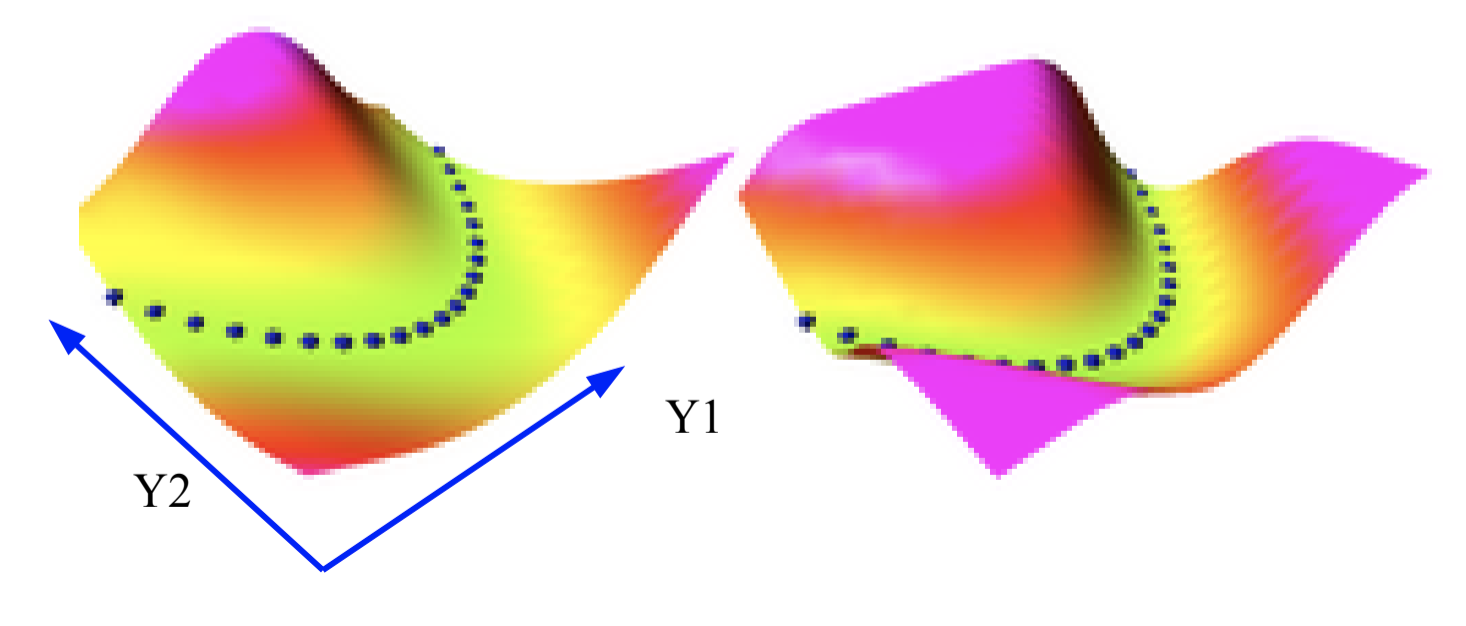
\includegraphics[width=100mm]{figs/pic2.png}
        \caption{Example: The samples live in the manifold}
        \label{figure1}
    \end{figure}
Making the energy low on the samples is easy (through back-propagation). But how do we make it high everywhere else? Pulling up the energies of unobserved points in high dimensional spaces is often very difficult and even intractable. 
Probabilistic models use a particular method for pulling up the energy of unobserved points that turn out to be very inefficient in many cases.

\subsection{Strategies to Shape the Energy Function}
% Authors: Kevin Ayuque (Editor), Bin Wang, Ding Wang
% Lecture date: 4/15/2019 part 2

\subsubsection{Build the machine so that the volume of low energy stuff is constant (PCA, K-means, GMM, square ICA)}

When it is known that the volume in the $y$ space of the machine can give limited energy (or maybe just constant). 
Normalized probabilistic models are of this type, if we increase the probability at one point, we have to decrease it at other points.
In other words, if we decrease the negative log probability at one point, we have to increase it at other points to maintain the normalization of the distribution. 
The whole volume of the probability is constant, equal to 1, which means that the volume of the low energy stuff is constant as well. Some normalized models that obeys this condition are Gaussian Mixture Model and PCA. On K-means the volume is not constant, it's bounded, so it does not fully obey this condition. 

The architecture of PCA is shown in Figure \ref{figure2}. The energy function is:
\begin{equation}
E(y,z) =  \norm{y-wz}^2,
\end{equation}
where $z$ belongs to the one hot vector. Then we compute the function 
\begin{equation}
F(y) =  min_z E(y,z).
\end{equation}
By changing $z$, we are selecting the column of $w$ that is closest to $y$ by doing this minimization.

\begin{figure}[H]
    \centering
    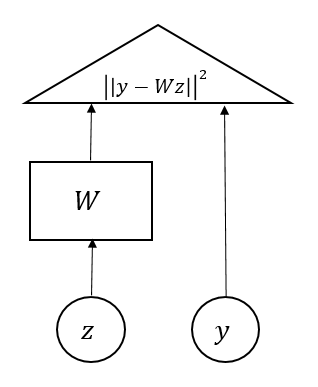
\includegraphics[width=0.35\textwidth]{figs/pic7.png}
    \caption{The architecture of PCA}
    \label{figure2}
\end{figure}

The architecture for K-means clustering has no encoder, only a decoder and a reconstruction cost module. 
The energy function of K-means is shown in Figure \ref{figure3}, as $y$ moves away from each prototype, the energy goes quadratically. 
The volume that can take low energy is limited by $k$. 
The only points that are reconstructed with zero energy are the prototypes. Every other point has higher energy.

 \begin{figure}[H]
    \centering
    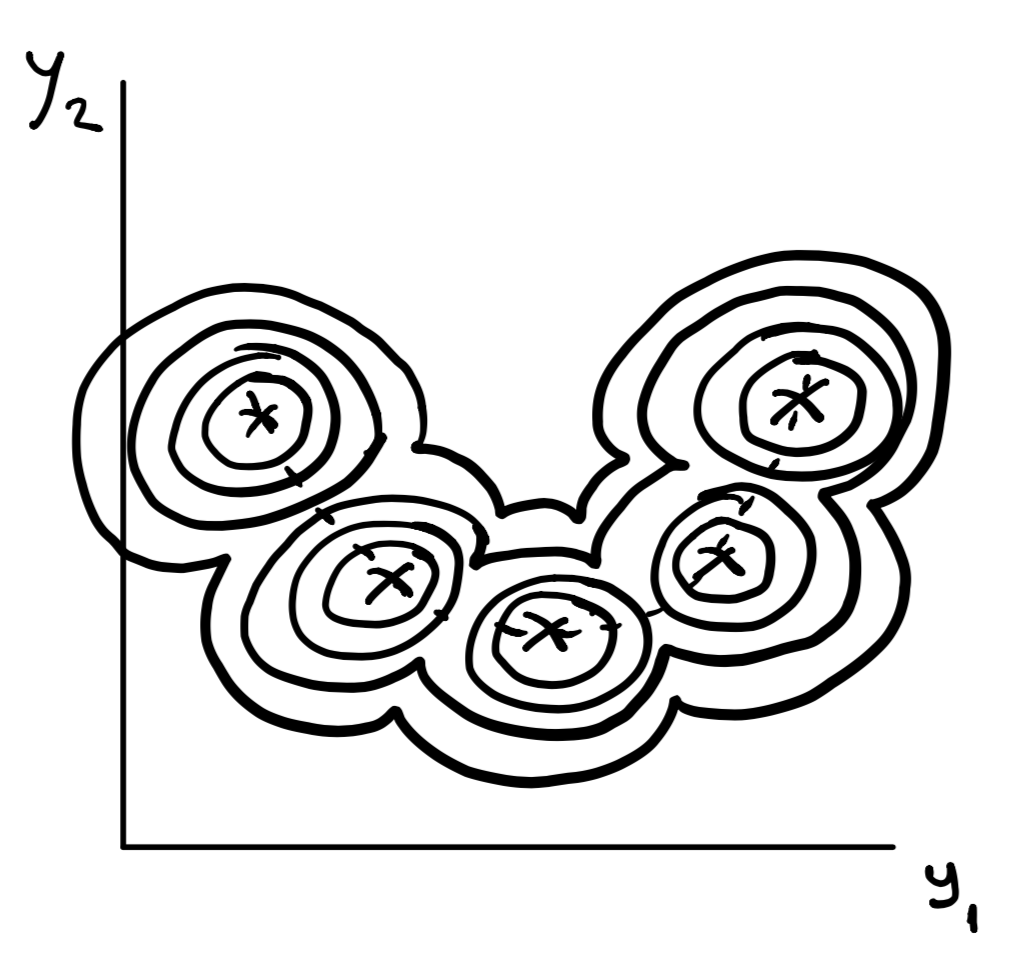
\includegraphics[width=0.5\textwidth]{figs/pic9.png}
    \caption{Energy function of k-means}
    \label{figure3}
\end{figure}

In Figure \ref{figure4}, the grey level represents energy, dark indicates low energy. 
Use the PCA as example, PCA avoids flat energy surface by using a code with a lower dimension than the input. 
Minimize the distance of every point with the projection, in this example is basically fitting a line to these points. 
The volume that can take low energy in PCA is limited, only a linear subspace of the input can have low energy, everything outside the subspace will have higher energy. 

PCA:
\begin{equation}
E(y,z) =  \norm{W^\top WY -Y}^2
\end{equation}

K-Means
\begin{equation}
E(Y) =  min_z \sum_i\norm{Y-W_iZ_i}^2
\end{equation}

\begin{figure}[H]
    \centering
    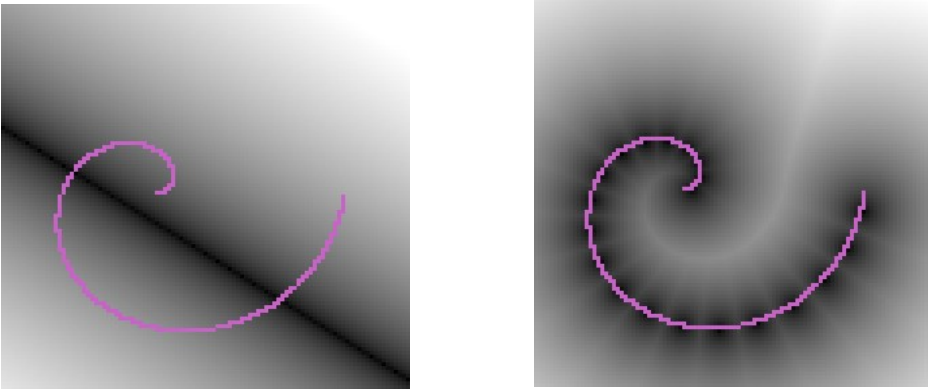
\includegraphics[width=\textwidth]{figs/pic1.png}
    \caption{Left: PCA and Right: K-Means}
    \label{figure4}
\end{figure}
   
\subsubsection{Push down of the energy of data points, push up everywhere else (Max likelihood (needs tractable partition function))}
    
This what full-fledged probability methods are doing. The probability of a point $y$ is given by Gibbs distribution which is derived from the energy function:
\begin{equation}
    P(Y|W) = \frac{e^{-\beta E(W,Y)}}{\int_y e^{-\beta E(W,y)}}
\end{equation}

Where $\beta$ is an arbitrary positive constant.
Training a probabilistic density model from a training dataset is generally performed by finding the $W$ that maximizes the likelihood of the training data under the model$ \sum^p_{i=1}P(Y^i,W)$. 
Equivalently, we can minimize a loss function $L(W,T)$ that is proportional to the negative log probability of the data. 
Here what we want to do is to minimize the negative log likelihood $L(W,T)$  on the training samples.

\begin{equation}\label{eq177}
    L(W,Y) = \frac{1}{p}\sum^p_{i=1}E(Y^i,W)+\frac{1}{\beta}log\int_y e^{-\beta E(y,W)}
\end{equation}

The gradient of $L(W,T)$ is

\begin{equation}
    \frac{\partial L(W,Y)}{\partial W}= \frac{1}{p}\sum^p_{i=1}\frac{\partial E(Y^i,W)}{\partial W}-\int_y P(y,W)\frac{\partial E(y,W)}{\partial W}
\end{equation}

In other words, minimizing the first term in equation \ref{eq177} with respect to $W$ has  the effect of making the energy of observed data points as small as possible, while minimizing the second term has the effect of “pulling up” on the energy of unobserved data points to make it as high as possible, particularly if their energy is low (their probability
under the model is high).

Naturally, evaluating the derivative of the second term in equation \ref{eq177}  may be intractable when Y is a high dimensional variable and $E(Y, W)$ is a complicated function for which the integral has no analytic solution. 
The intractable integral is often evaluated through:

\begin{itemize}
    \item Monte-Carlo sampling, where we are going to replace the integral with discrete sum, where we draw samples from the distribution and then compute the average of the samples.
    \item Variational approximations, where we replace the distribution $P$ with one that we know how to compute, like Gaussian. 
    So we pick Gaussian which is possible the best approximation to $P$, in terms of KL Divergence, which measures the divergence between distributions. 
    We replace P by Q, and then compute $(17.8)$, while minimizing the divergence between P and Q at the same time.
\end{itemize}

\subsubsection{Push down of the energy of data points, push up on chosen locations (contrastive divergence, Ratio Matching, Noise Contrastive Estimation, Minimum Probability Flow)}

Monte Carlo methods, adversarial training, generative adversarial networks and many more falls under this category.
 
\subsubsection{Minimize the gradient and maximize the curvature around data points (score matching)}

The idea is to take the energy function and try to make it flat around data points.
In other words, we want the gradient of the energy function in $y$ space (with respect to input $y$) to be $0$, because we want the energy to be minimum. 
See figure \ref{figure8} . 
The ideal energy function is the one that take low values around the points and value increases as we move away. 
In other words we can define score matching as having an energy function that has zero gradient with respect to the input, while also having a second derivative that is as large as possible. 
However, the problem is that we have to compute the gradient of the trace of the Hessian with respect to the parameters. 
This idea is \textit{"cute but impractical"}, except for very simple models. 

\begin{figure}[htb]
    \centering
    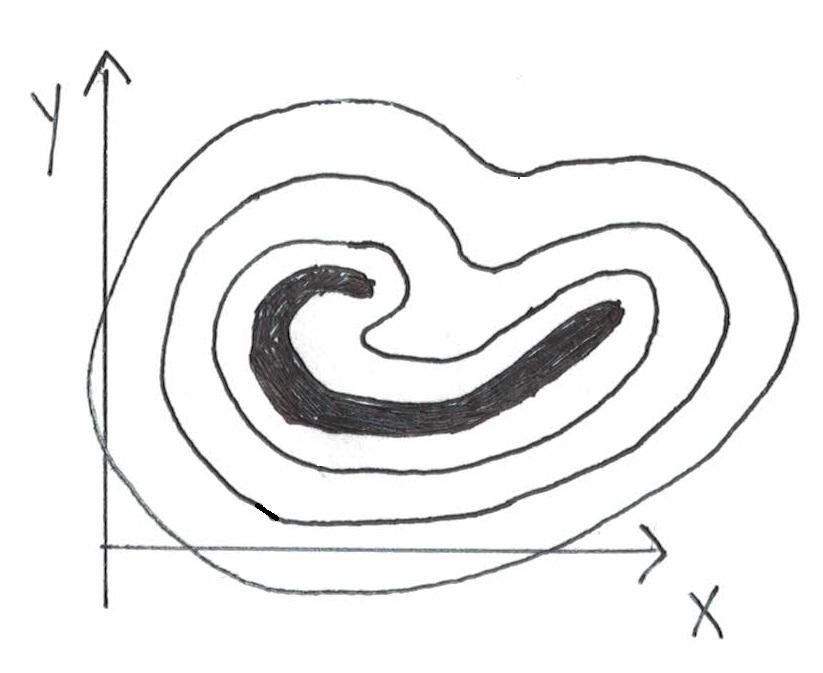
\includegraphics[width=0.35\textwidth]{figs/pic8.png}
    \caption{Energy Function}
    \label{figure8}
\end{figure}

\subsubsection{Train a dynamical system so that the dynamics goes to the manifold (denoising auto-encoder)}

The idea of denoising auto-encoder is very useful. 
We start with the raw input $y$, and corrupt it with some noise, and then run it through some parameterized function $G_w(y)$. 
Then we take the uncorrupted input and compute the distance with the output from the function $G_w(y)$. 
By applying corruption and function $G_w(y)$, we are supposed to reconstruct the original $y$ with its prediction $\bar y$. 
Then we minimize the reconstruction error, which is the square of distance between $\bar y$ and $y$.
See \ref{figure6}. 
In other words, the function $G_w(y)$ maps the point outside the manifold to the point inside the manifold. 
At test time, we remove the corrupt part and give a $y$ without corruption. 

The energy-based view of denosing auto-encoder is that when we train the function to map the points outside the manifold to the points on the manifold, we train it to compute the energy, which is the reconstruction error.

Two slight problems remain:

\begin{itemize}
    \item We don't know what noise, or what types of corruptions make sense.
    \item There are many ways that one can corrupt an input in the high dimensional space.
    We may not be able to cover all possible ways to corrupt an input that can span the high dimensional space. 
    Besides, there is no guarantee that the model learns exactly what we teach it. It may not be able transform all the points to the manifold.
\end{itemize}

\begin{figure}[htb]
    \centering
    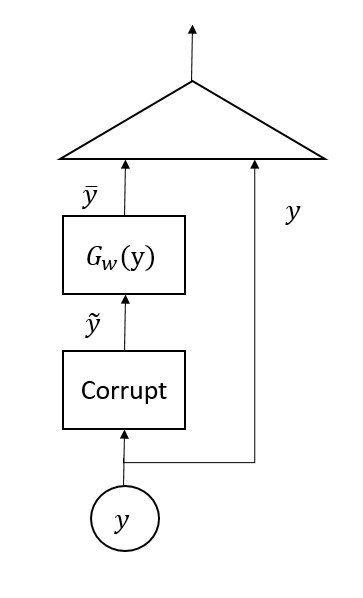
\includegraphics[width=0.35\textwidth]{figs/PIC6.PNG}
    \caption{The architecture of denoising auto-encoder}
    \label{figure6}
\end{figure}

\subsubsection{Use a regularizer that limits the volume of space that has low energy}
This will be discussed in more detail on April 29.
    
\subsubsection{If $E(Y) = ||Y - G(Y)||^2$, make $G(Y)$ as "constant" as possible.(Contracting auto-encoder, saturating auto-encoder)}

Contracting auto-encoder comes from Yoshua Bengio's lab. Basically, it's still in the architecture of auto-encoder in figure  \ref{figure5}.

\begin{figure}[htb]
    \centering
    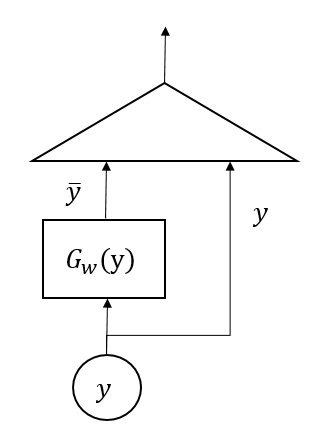
\includegraphics[width=0.35\textwidth]{figs/PIC5.PNG}
    \caption{The architecture of auto-encoder}
    \label{figure5}
\end{figure}

The energy of $y$ is $$ E(y) = ||y-G(y)||^2, $$ and the loss function is $$L = \sum_i E(y^i)+R(w),$$ where the regularization term $R(w)$ is the square Frobenius norm of Jacobian of the hidden layer representation with respect to input values. 
This encourages a constant hidden representation except around training samples where it is counteracted by the reconstruction term.
